\section{Methodology}

The first methodological step was fetching the different datasets on Sentinel-2 images, tree locations and OSM information which was then input into a U-Net deep learning model. The system then predicts tree locations on unseen satellite images and validates performance while accounting for risks such as image quality and seasonal variation. Figure~\ref{fig:overview_beam} shows this process.

\begin{figure}[H] 
    \centering
    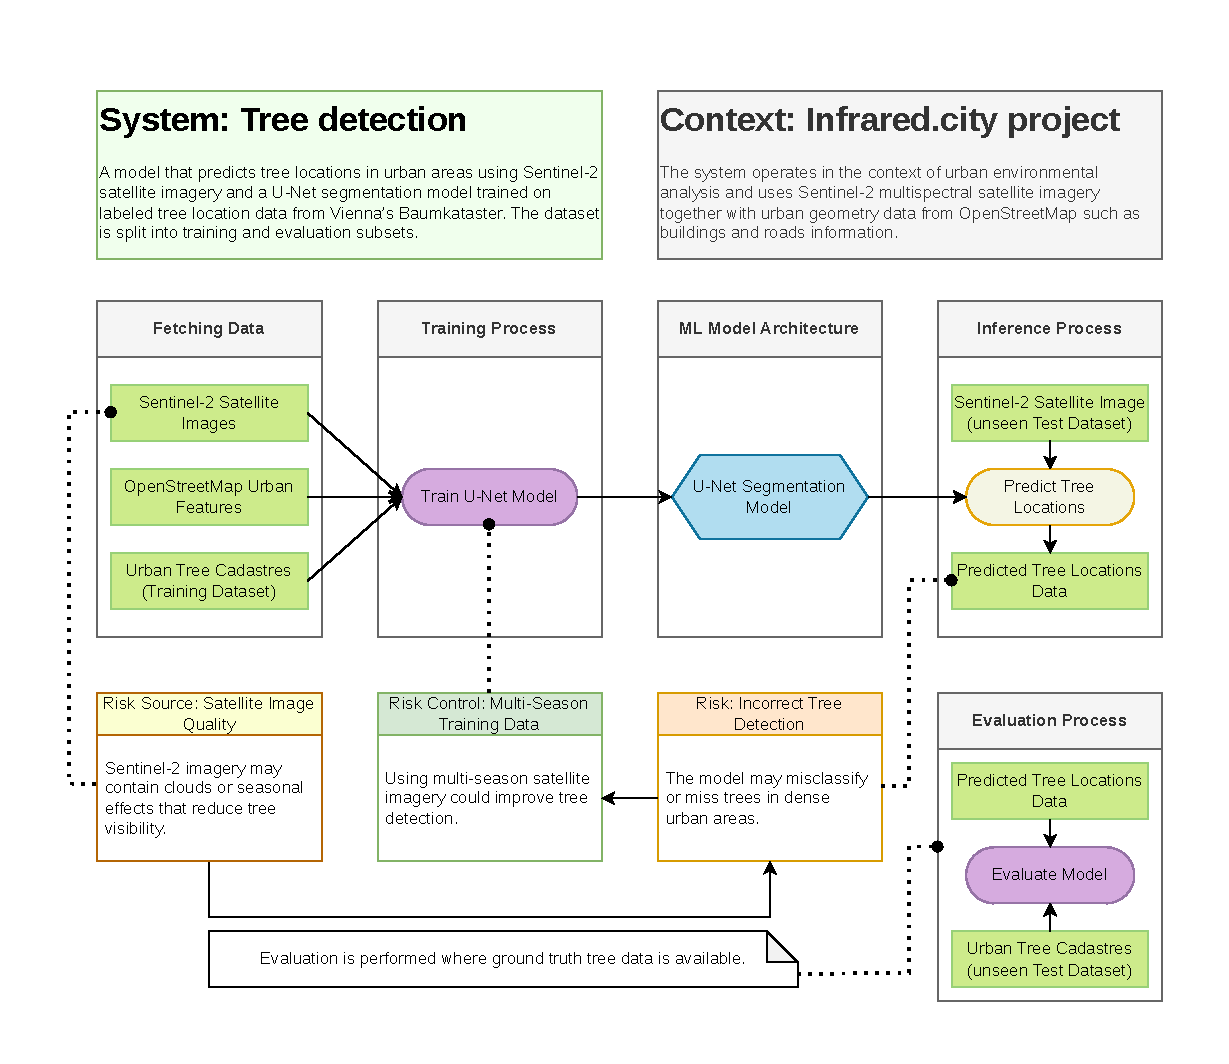
\includegraphics[width=\textwidth]{images/refined_beam_treeDetection_infraredCity.drawio.pdf}
    \caption{BEAM model of the proposed tree detection system.}
    \label{fig:overview_beam}
\end{figure}

\subsection{Model}

For this tree detection task we implemented a U-Net regression architecture with a temporal attention mask which predicts the number of trees per pixel of Sentinel-2 data where the prediction labels are derived from communal tree registries. 

Former papers suggest that for image segmentation using satellite data the U-Net deep learning model is the most accurate for detecting objects, for example street detection \cite{pesek2024convolution} as well as crop field detection \cite{garnot2021panoptic}. 
Furthermore, last year's \textit{infrared.city} project also tried implementing a U-Net architecture but failed to yield promising results, also the data coaches deem it a well-fitting model. 

In Figure~\ref{fig:unet_beam}  the U-Net model is a special type of Convolutional Neural Network and consists of a contracting path and an expanding path.
First, the satellite image is put through an input convolution so it has the correct structure for further processing.
It is then passed into the contracting path to down-sample the data in the convolution and pooling layers, which are used to extract features from the original imagery. 
Our model uses four convolutional layers where during contraction for each layer the image size gets smaller due to pooling meanwhile evermore features are extracted from the images. The same process happens vice versa for the expansionary path. The expanding path consists of the same structure of convolution and pooling layers but this time used to up-sample the before contracted imagery \cite{aramendia2024}. 
To get the final prediction of the number of trees per pixel another convolutional layer is deployed. 
As suggested in similar work this project will use skip connections between the expanding and contracting path as well as a temporal attention algorithm to prioritize more meaningful images \cite{garnot2021panoptic} and take advantage of the seasonality and changing vegetation of trees.
The model uses smoothed L1 loss (also called Huber loss) and the tree registry data as a ground truth.

\begin{figure}[H] 
    \centering
    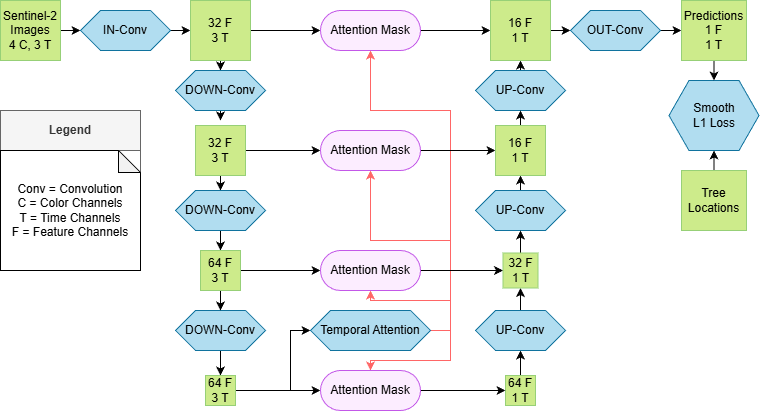
\includegraphics[width=\textwidth]{images/U-Net.png}
    \caption{U-Net Model}
    \label{fig:unet_beam}
\end{figure}